%************************************************
\chapter{Results and Discussion}
\label{chp:results}
%************************************************

\textbf{The different evaluation methods somehow complete one another since they take different aspects into account...} lägg till detta någonstans...

%========================================================================%
\section{Map generation- Use entire data set}
%========================================================================%

Figure \ref{fig:results/ch_all} displays the two generated maps C1m and C7m described in section \ref{chp:experimental_setup.sec:mapgen}. The maps are plotted in blue and are put on top of Google Maps in the area of interest. 

By simply looking at the figures, the maps looks quite accurate. Note though, that the current state of the art inferred maps have incomplete coverage and imperfect topological structure \citep{fuse}. In the following sections we will evaluate the maps using the three proposed evaluation methodologies in section \ref{chp:method.sec:evaluation}. The maps are in these evaluation methods compared to the ``verified'' ground truth \ac{OSM} of the Chicago 1 month and 7 month data sets, see figure \ref{fig:data/osmdata} in section \ref{chp:data.sec:osm.sec:gt}. In this section, only data from the Chicago data sets will be used, see section \ref{chp:data.sec:gpsdata.sec:chicago}. 

% Google maps
\begin{figure}%
 \centering
 
 \subfloat[\textit{\textit{Chicago 7 month data set.}}]{{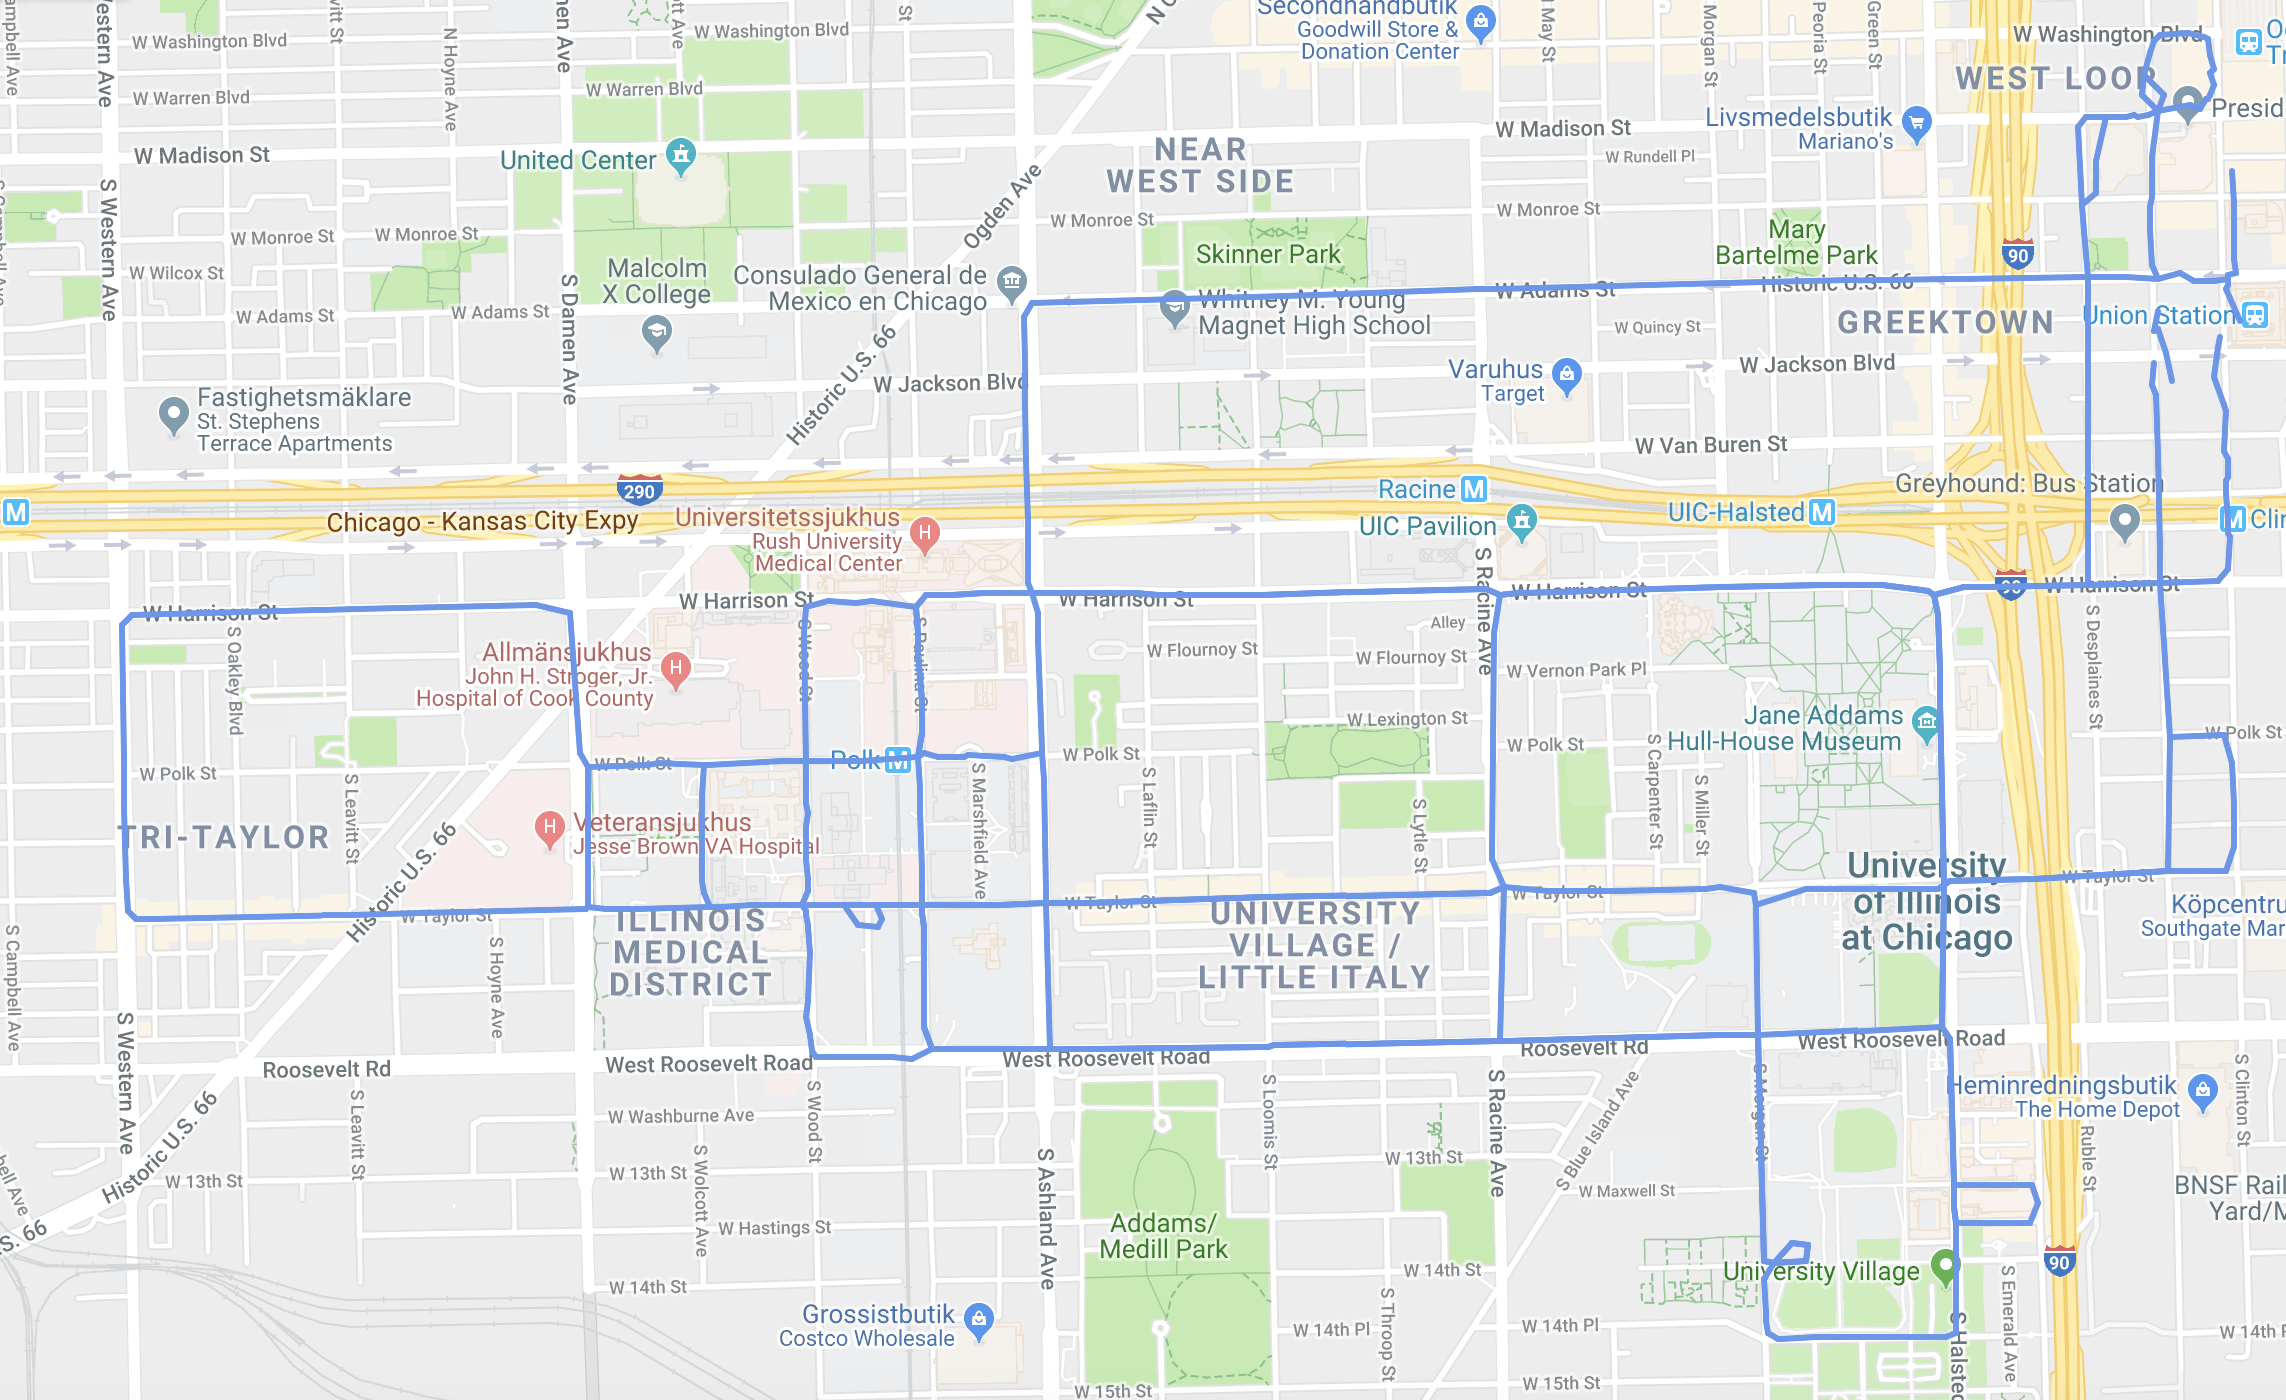
\includegraphics[width=\linewidth]{Figures/Results/chicago/maps/chicago_1m.png}\label{results/ch1m} }}%
 
  \subfloat[\textit{Chicago 7 month data set.}]{{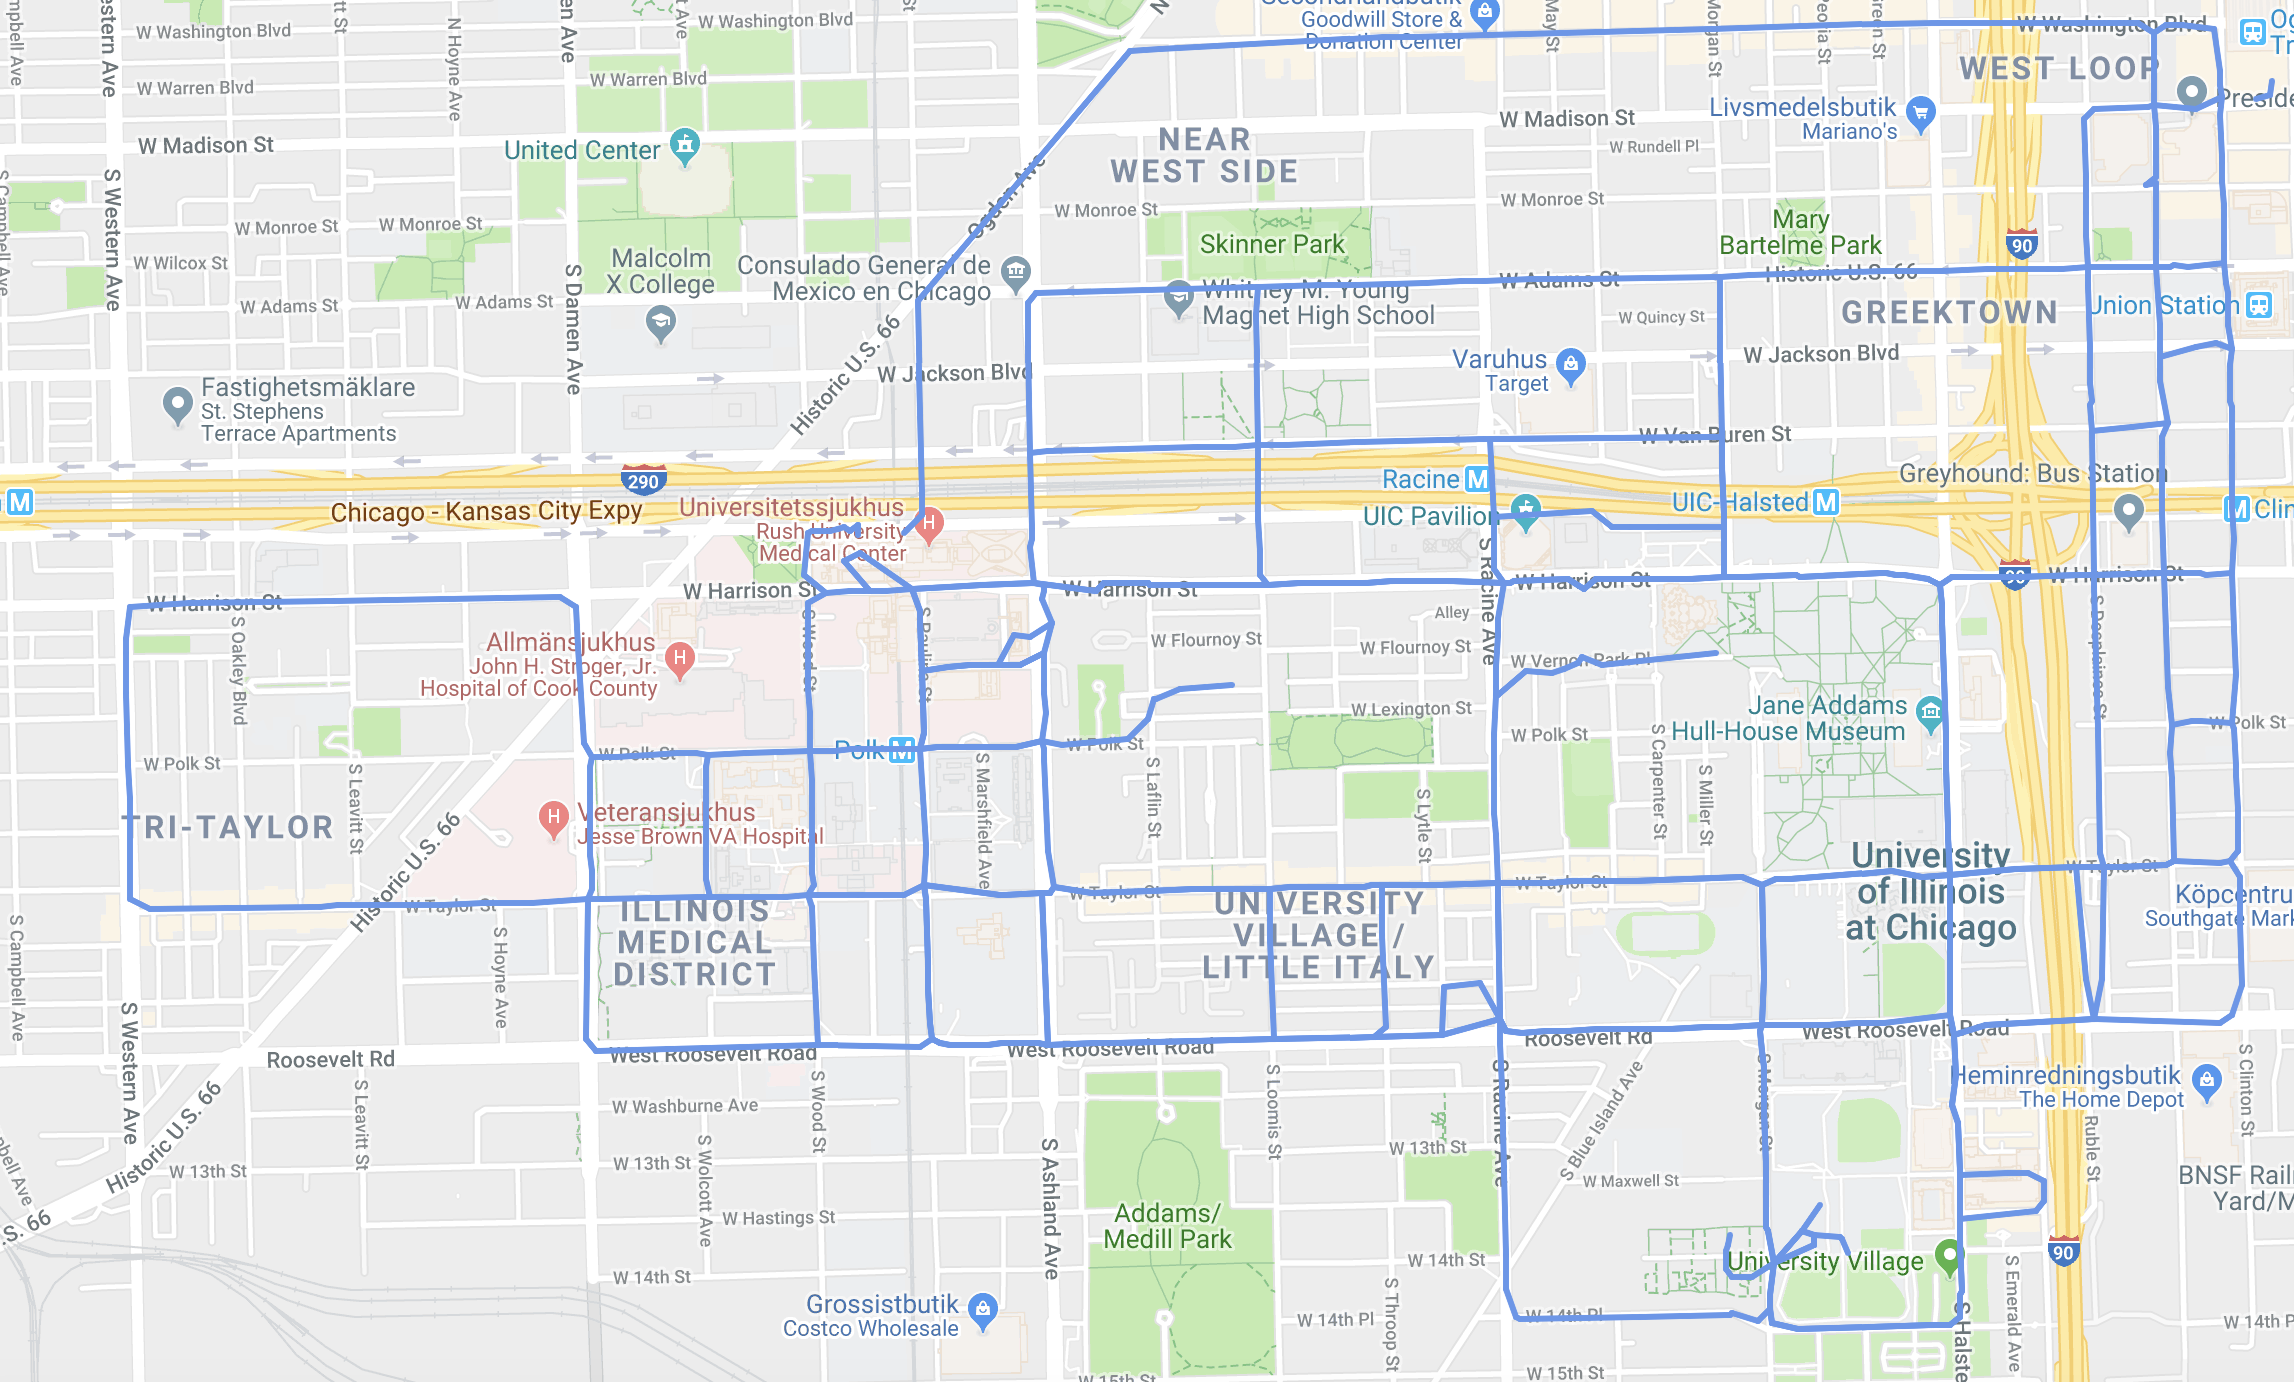
\includegraphics[width=\linewidth]{Figures/Results/chicago/maps/chicago_7m.png}\label{fig:results/ch7m} }}%

 \caption{Generated maps for the Chicago data sets on top of Google maps in the area of interest.}%
 \label{fig:results/ch_all}
\end{figure}



-------temporary to know what to do-------
\begin{table}[H]
\centering
\caption{Summary of map generation experiments.}
\label{tab:hskhjsjksjk}
\begin{tabular}{ccc}
\begin{tabular}[c]{@{}c@{}}map generation\\ experiment\end{tabular} & base map   & new map \\ \hline
MG1                                                                 & COSM12\_1m & C1m     \\
MG2                                                                 & COSM12\_7m & C7m     \\
MG3                                                                 & C1m        & C7m     \\
MG4                                                                 & C7m        & C1m     \\ 
MG5                                                                 & COSM12     & COSM18  \\ \hline
\end{tabular}
\end{table}
------------------------------------------
\textbf{ha en till kolonn som heter $map_gen_exp_1$ osv? hur ska vi skriva om de olika experimentet? allt huller om buller eller ett i taget??}

%------------------------------------------------------------------------%
\subsection{Using OSM as ground truth}
%------------------------------------------------------------------------%
%Here we evaluate our created maps to the ``ground truth" OSM.


%........................................................................%
\subsubsection{GEO}
%........................................................................%
In figure \ref{fig:results/geo_match_dist_ch} the result of the geometric evaluation is shown when comparing against the ground truth maps, COSM12\_1m and COSM12\_7m. As motivated in section \ref{ch:experiments.sec:paramtuning} the sample spacing is fixed to 5 m. The matching distance between markers is varied from 1 to 100 meters.

The precision of the generated roads approaches 1 as the matching threshold is increased. However, recall remains around 0.8. In some cases we infer a road that lies in between two close roads in the \ac{OSM}. For this road, precision will be high while recall is low. As the F-score is the harmonic mean between these two it is a more accurate measure of the performance of the method for these cases. Since there are also some missing roads in the inferred map the score of the generated map will not be perfect even with a very large threshold.

% geo1
\begin{figure}[H]%
  \mycenter{
  \subfloat[\textit{Chicago 1 month data set.}]{ 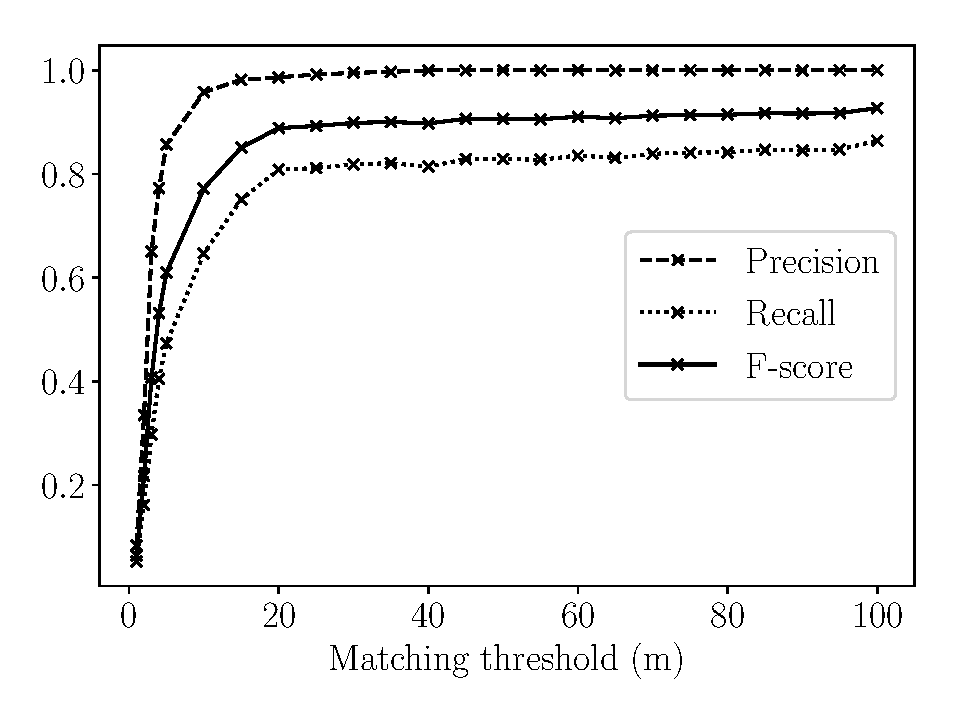
\includegraphics[width=0.6\linewidth]{Figures/Results/chicago/geo/match_dist_chicago_1m.pdf}\label{fig:results/geo_match_dist_ch1m} }% 
  \subfloat[\textit{Chicago 7 month data set.}]{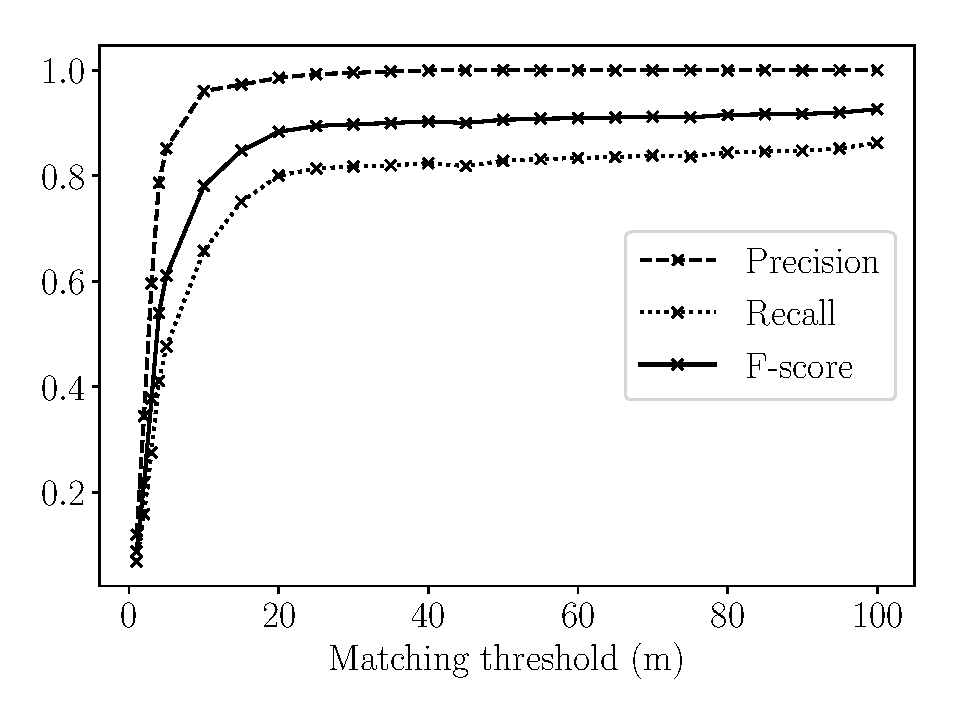
\includegraphics[width=0.6\linewidth]{Figures/Results/chicago/geo/match_dist_chicago_7m.pdf}\label{fig:results/geo_match_dist_ch7m} }%
  }
  \caption{GEO evaluation of the Chicago data sets using COSM\_1m and COSM\_7m as ground truth. The matching distance is varied from 1 to 100 meters and the sample spacing fixed to 5 m.}%
 \label{fig:results/geo_match_dist_ch}
\end{figure}


%........................................................................%
\subsubsection{TOPO}
%........................................................................%
The same experiment was run using the TOPO evaluation metric. As motivated in section \ref{ch:experiments.sec:paramtuning} we fix the sample spacing at 5 meters, the number of evaluations per evaluation run at 150 and the max sampling distance at 300 m. 

We can see from figure \ref{fig:results/topo_match_dist_ch} that both precision and recall is now lower compared to the GEO evaluation. This is a result of now taking both direction and connectivity of the roads into account in the evaluation. Topological differences between the maps is now penalised which results in a more accurate measure of the quality of the generated map.

% topo
\begin{figure}[H]%
 \mycenter{

  \subfloat[\textit{\textit{Chicago 1 month data set.}}]{{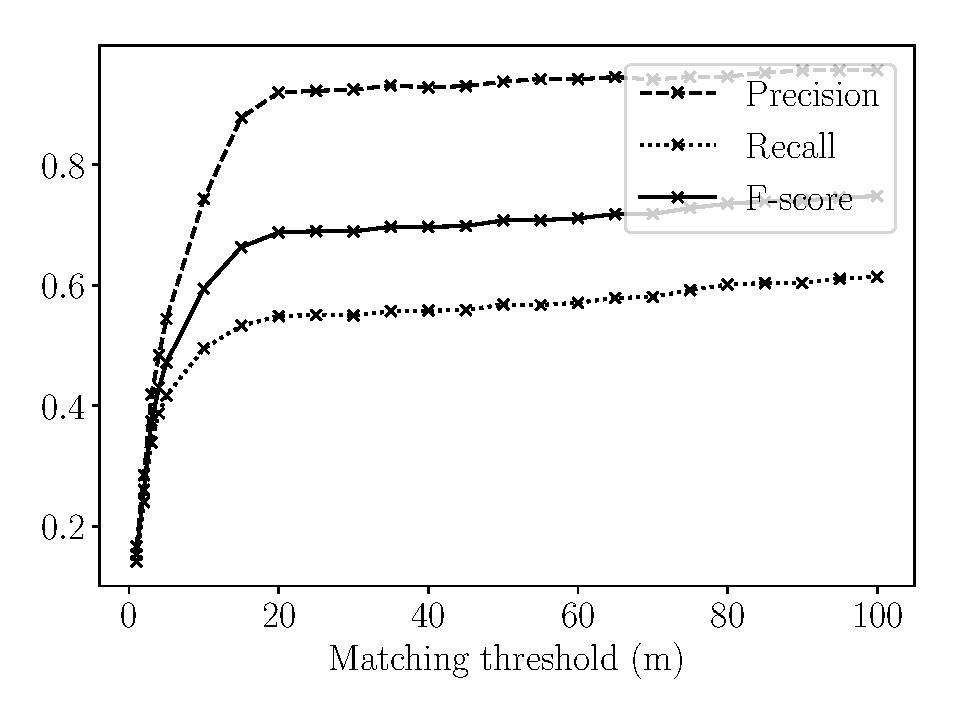
\includegraphics[width=0.6\linewidth]{Figures/Results/chicago/topo/match_dist_chicago_1m.pdf}\label{fig:results/topo_match_dist_ch1m} }}% 
  \subfloat[\textit{Chicago 7 month data set.}]{{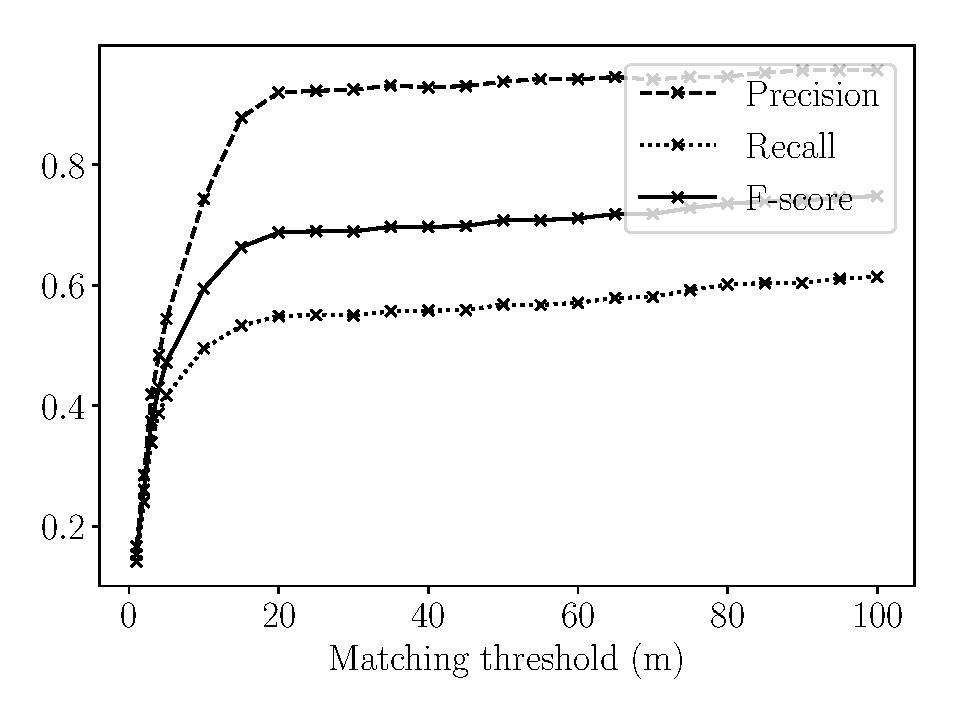
\includegraphics[width=0.6\linewidth]{Figures/Results/chicago/topo/match_dist_chicago_7m.pdf}\label{fig:results/topo_match_dist_ch7m} }}%
  }
  \caption{TOPO evaluation of the Chicago data sets. The matching distance is varied from 1 to 100 meters.}%
 \label{fig:results/topo_match_dist_ch}
\end{figure}

Further, the TOPO evaluation metric was used to compute the local signature of each edge in the maps as described in section \ref{chp:method.sec:evaluation.sub:topo}. The result for the Chicago 1 month and 7 month data sets can be seen in figure \ref{fig:results/sig_topo_1m} and \ref{fig:results/sig_topo_7m} respectively. The value of the local signature for an edge lies in the interval 0 to 1, since it will be the F-score of the neighbourhood of an edge. The colour bar will range from red, corresponding to a low F-score to green, meaning a high F-score and high similarity between maps. Since we are here comparing to ground truth, edges with a low local signature in the inferred map will correspond to low confidence areas.

This metric can be used to detect differences between maps. These differences could correspond to either missing roads or new roads. In the hospital area in the top right corner map C1m has a few noisy roads where the roads are disconnected. This is captured in the signature for the edges in this area, as the topology of C1m compared to COSM\_1m will be different here.

% topo edge sign
\begin{figure}[H]%

 \subfloat[\textit{\textit{C1m as base map.}}]{{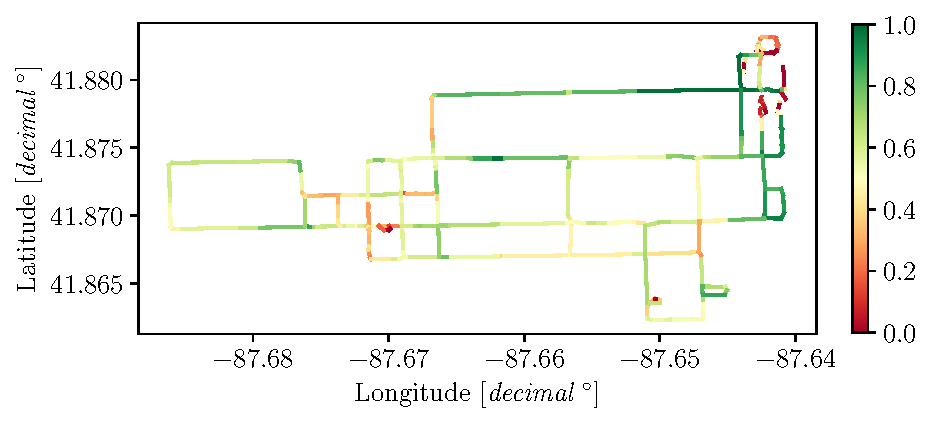
\includegraphics[width=0.8\linewidth]{Figures/Results/chicago/topo/local_signatures_chicago_1m.pdf} }}%
 
  \subfloat[\textit{COSM12$\_$1m as base map.}]{{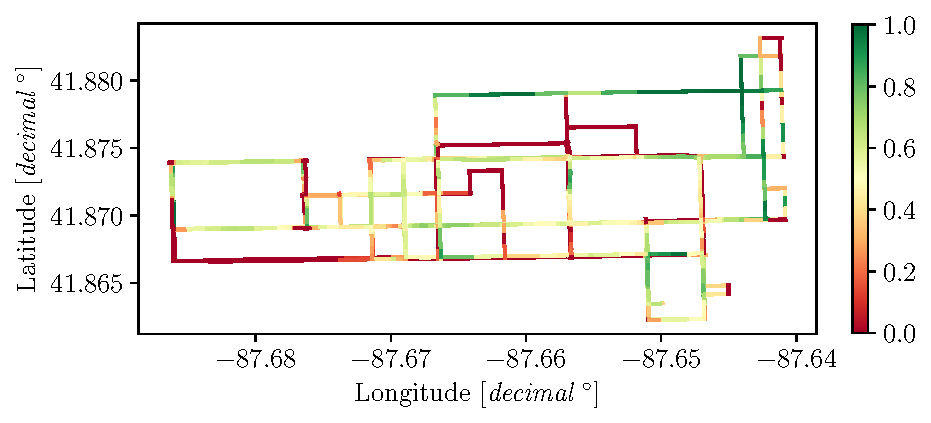
\includegraphics[width=0.8\linewidth]{Figures/Results/chicago/topo/local_signatures_chicago_osm_1m.pdf} }}%
  
 \caption{Edge signatures for maps C1m and COSM12$\_$1m calculated using TOPO.}%
 \label{fig:results/sig_topo_1m}
\end{figure}

\enlargethispage{5\baselineskip}

% topo use inferred as base map
\begin{figure}[H]%

 \subfloat[\textit{\textit{C7m as base map.}}]{{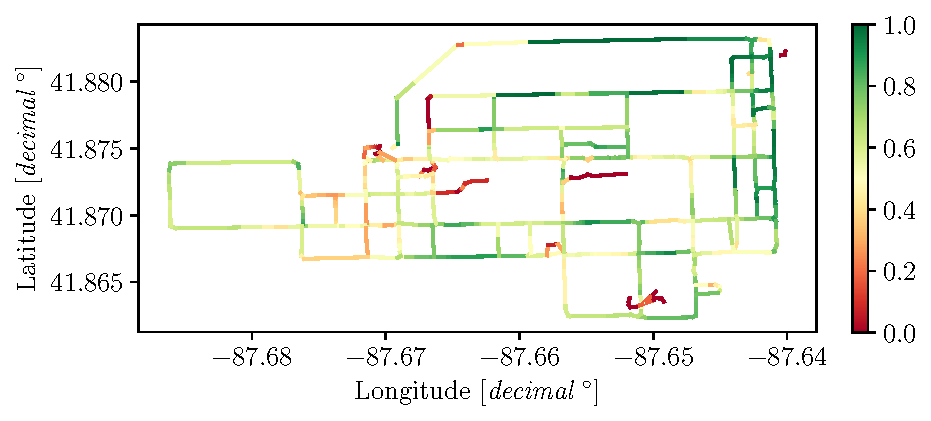
\includegraphics[width=0.8\linewidth]{Figures/Results/chicago/topo/local_signatures_chicago_7m.pdf}}}%
 
  \subfloat[\textit{COSM12$\_$7m as base map.}]{{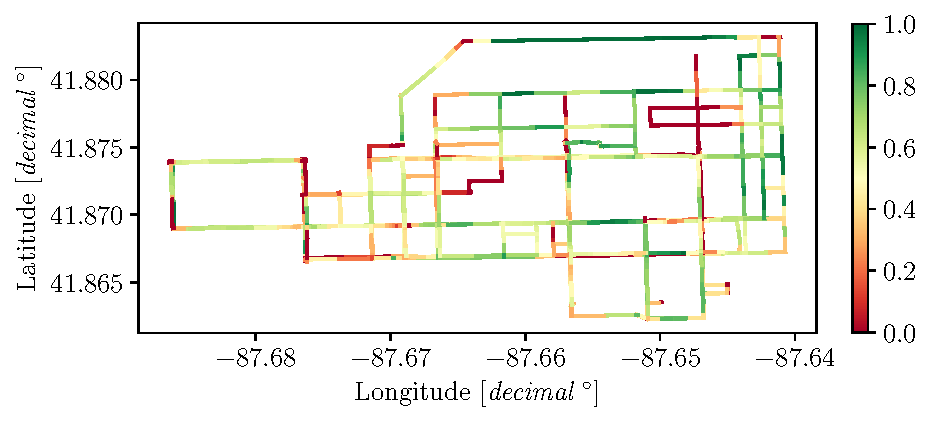
\includegraphics[width=0.8\linewidth]{Figures/Results/chicago/topo/local_signatures_chicago_osm_7m.pdf} }}%
  
 \caption{Edge signatures for maps C7m and COSM12$\_$7m calculated using TOPO.}%
 \label{fig:results/sig_topo_7m}
\end{figure}



%........................................................................%
\subsubsection{Path based}
%........................................................................%


In figures \ref{fig:results/c1mosmpathl1}, \ref{fig:results/c1mosmpathl2} and \ref{fig:results/c1mosmpathl3} the edge signatures are plotted for maps C1m and COSM12$\_$1m using link length 1, 2 and 3 respectively. For the interested reader the corresponding edge signatures are plotted for maps C7m and COSM12$\_$7m in appendix \ref{chp:appendix:A1} in figures \ref{fig:results/c7mosmpathl1}, \ref{fig:results/c7mosmpathl2} and \ref{fig:results/c7mosmpathl3}. 

These figures displays in a illustrative manner which edges have a similar or non-similar neighbourhood surrounding it in the other map. It can therefore be seen as a type of change detection. The numbers in the colour bars corresponds to the local edge signatures explained in \ref{chp:method.sec:evaluation.sub:pathbased}.
We choose to plot the edge signatures this way once and will further on only plot the cumulative distribution.   

%\begin{changemargin}{-1cm}{-1cm}


\begin{figure}[H]%
 \centering
 
 \subfloat[\textit{\textit{C1m as base map.}}]{{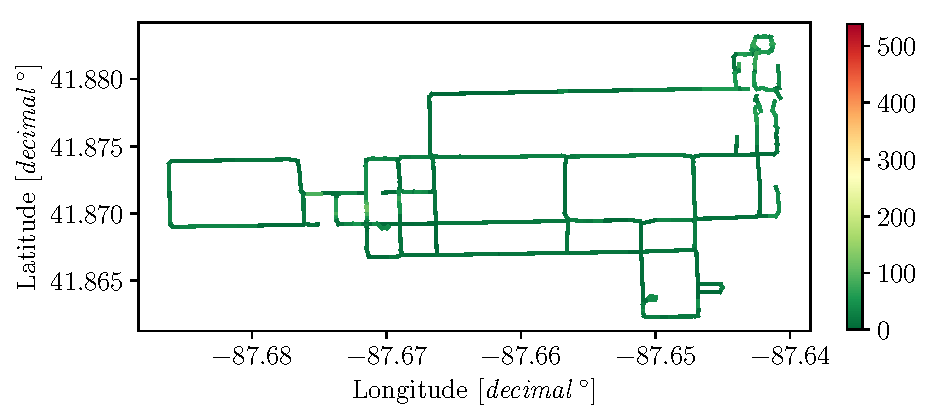
\includegraphics[width=0.8\linewidth]{Figures/Results/chicago/path_based/chicago_1m_chicago_osm_1m_link1.pdf}\label{fig:results/c1mosm1} }}%
 
  \subfloat[\textit{COSM12$\_$1m as base map.}]{{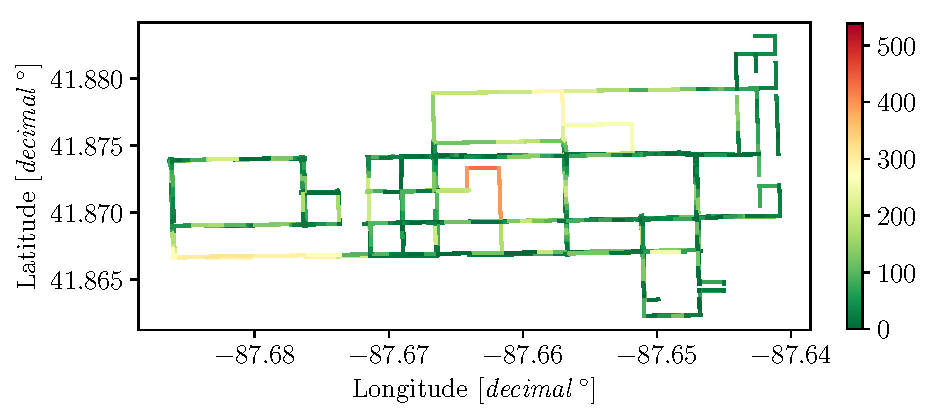
\includegraphics[width=0.8\linewidth]{Figures/Results/chicago/path_based/chicago_osm_1m_chicago_1m_link1.pdf}\label{fig:results/osmc1m1} }}%

 \caption{Edge signatures for maps C1m and COSM12$\_$1m using link length 1.}%
 \label{fig:results/c1mosmpathl1}
\end{figure}

\enlargethispage{5\baselineskip}

\begin{figure}[H]%
 \centering
  \subfloat[\textit{\textit{C1m as base map.}}]{{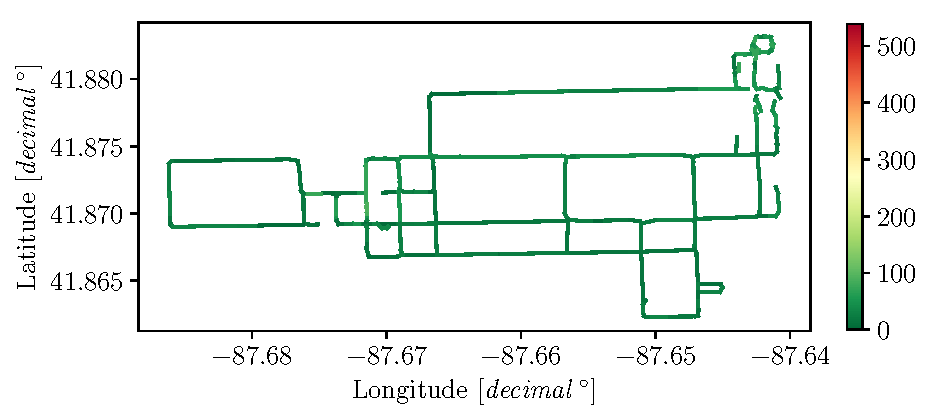
\includegraphics[width=0.8\linewidth]{Figures/Results/chicago/path_based/chicago_1m_chicago_osm_1m_link2.pdf}\label{fig:results/c1mosm2} }}% 

  \subfloat[\textit{COSM12$\_$1m as base map.}]{{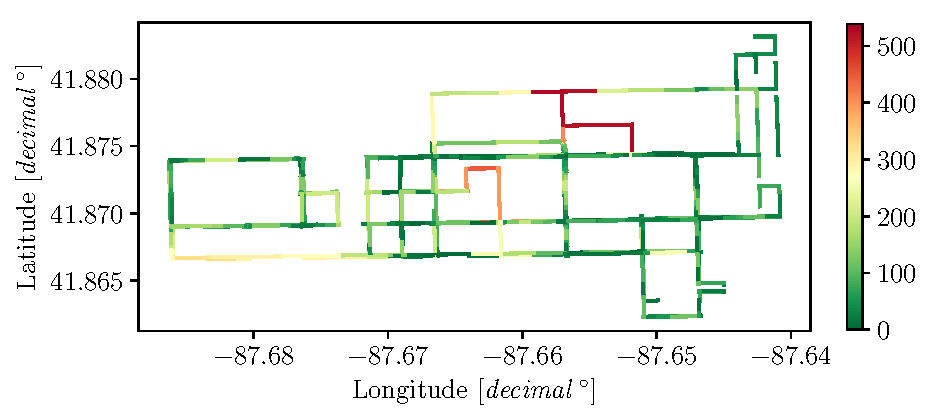
\includegraphics[width=0.8\linewidth]{Figures/Results/chicago/path_based/chicago_osm_1m_chicago_1m_link2.pdf}\label{fig:results/osmc1m2} }}%
  \caption{Edge signatures for maps C1m and COSM12$\_$1m using link length 2.}%
 \label{fig:results/c1mosmpathl2}
\end{figure}


%\end{changemargin}

\begin{figure}[H]%
 \centering
 
  \subfloat[\textit{\textit{C1m as base map.}}]{{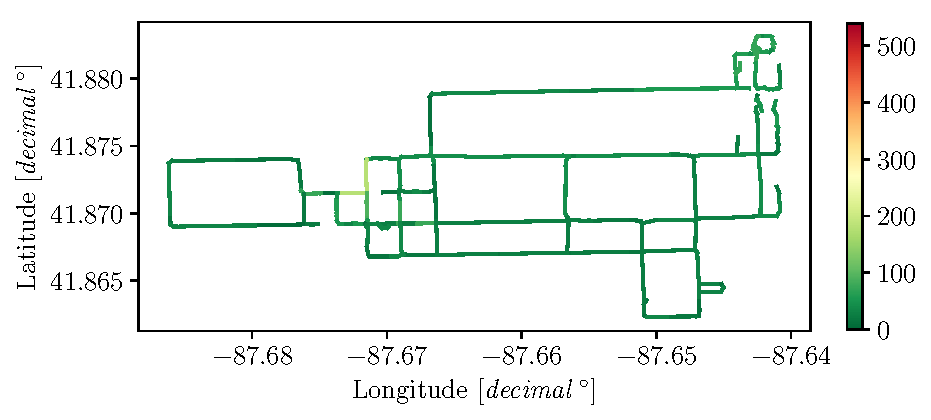
\includegraphics[width=0.8\linewidth]{Figures/Results/chicago/path_based/chicago_1m_chicago_osm_1m_link3.pdf}\label{fig:results/c1mosm3} }}% 

  \subfloat[\textit{COSM12$\_$1m as base map.}]{{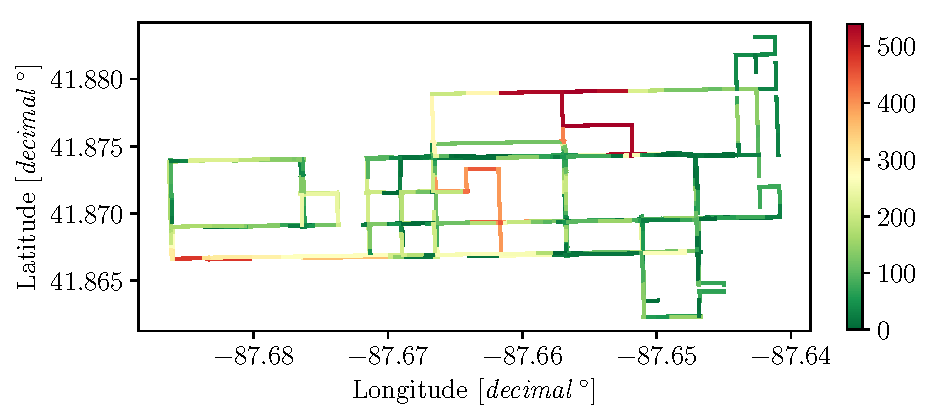
\includegraphics[width=0.8\linewidth]{Figures/Results/chicago/path_based/chicago_osm_1m_chicago_1m_link3.pdf}\label{fig:results/osmc1m3} }}%
  
  \caption{Edge signatures for maps C1m and COSM12$\_$1m using link length 3.}%
 \label{fig:results/c1mosmpathl3}
\end{figure}


\textbf{Let's discuss the results a bit further... }


%------------------------------------------------------------------------%
\subsection{Using inferred map as ground truth}
%------------------------------------------------------------------------%

\subsubsection{GEO}

Further, we present the result of evaluating map C1m against C7m and map C7m against C1m using GEO. We can in this case consider the previous inferred map to be ``ground truth''. The result can be seen in figure \ref{fig:results/geo_match_dist_chch}.
% geo2
\begin{figure}[H]%
  \mycenter{
  \subfloat[\textit{Chicago 1 month data set.}]{ 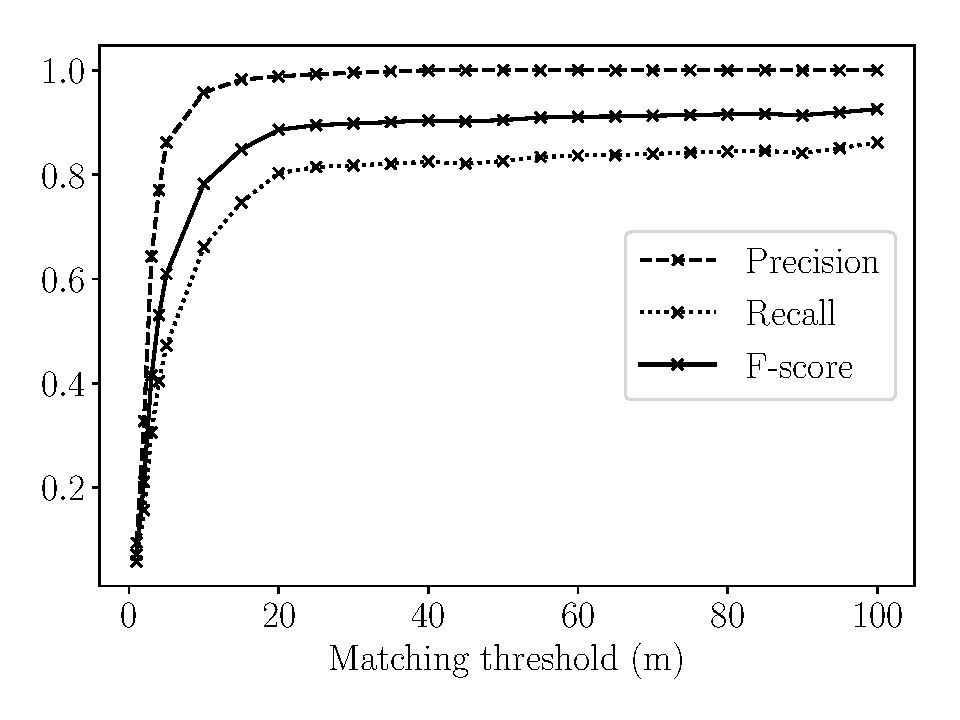
\includegraphics[width=0.6\linewidth]{Figures/Results/chicago/geo/match_dist_ch1ch7.pdf}\label{fig:results/geo_match_dist_ch1ch7} }% 
  \subfloat[\textit{Chicago 7 month data set.}]{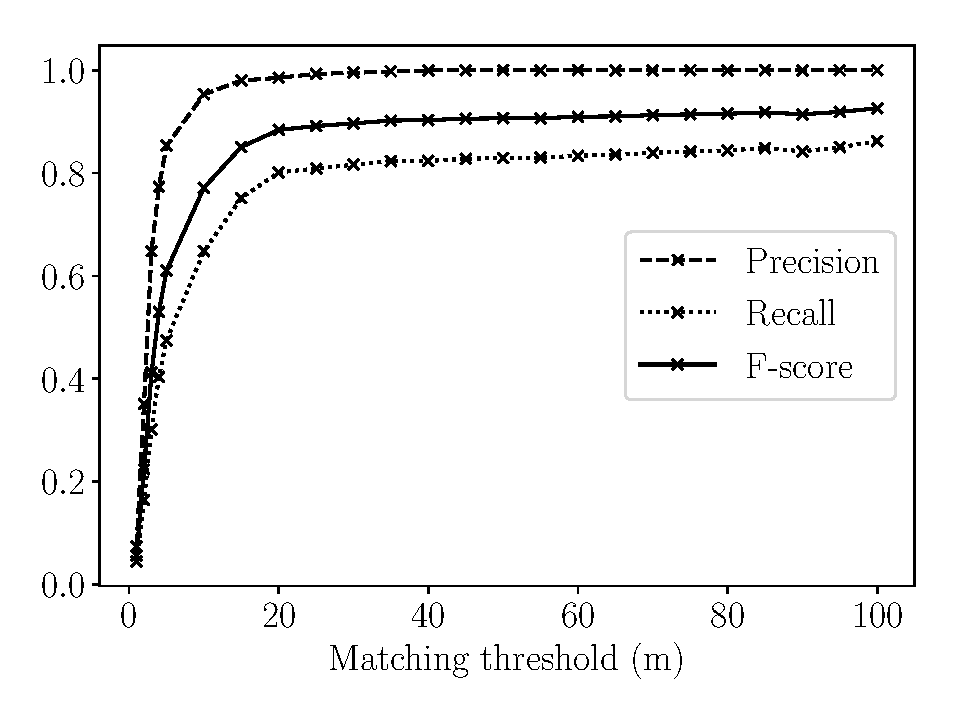
\includegraphics[width=0.6\linewidth]{Figures/Results/chicago/geo/match_dist_ch7ch1.pdf}\label{fig:results/geo_match_dist_ch7ch1} }%
  }
  \caption{TOPO evaluation of the Chicago data sets using C7m and C1m as ground truth. The matching distance is varied from 1 to 100 meters and the sample spacing fixed to 5 m.}%
 \label{fig:results/geo_match_dist_chch}
\end{figure}

\subsubsection{TOPO}

\begin{figure}[H]%
  \mycenter{
  \subfloat[\textit{Chicago 1 month data set.}]{ 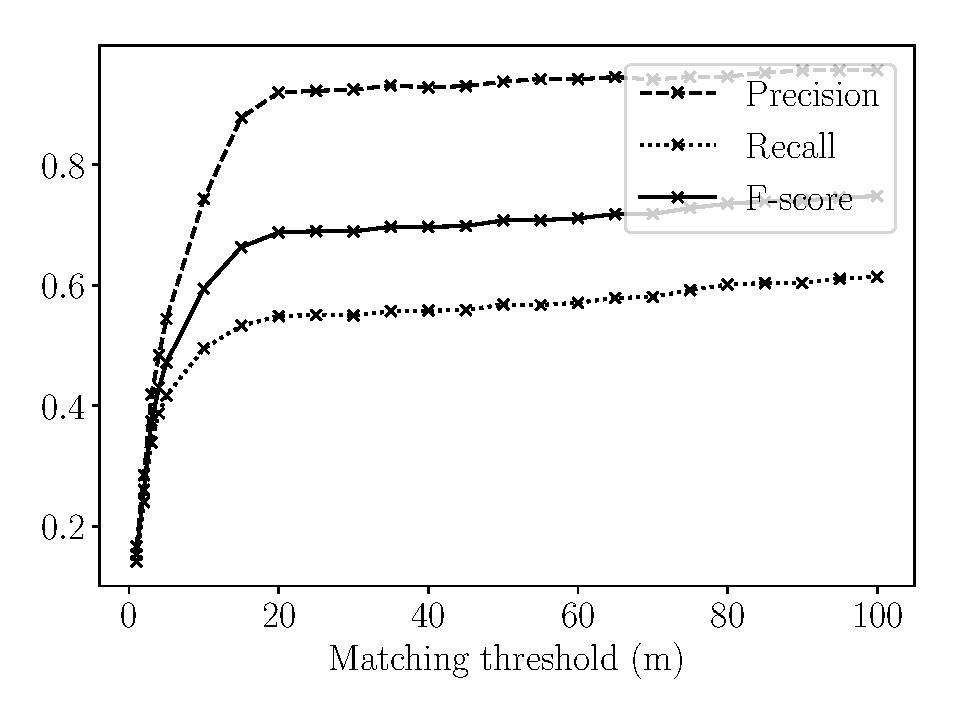
\includegraphics[width=0.6\linewidth]{Figures/Results/chicago/topo/match_dist_ch1ch7.pdf}\label{fig:results/topo_match_dist_ch1ch7} }% 
  \subfloat[\textit{Chicago 7 month data set.}]{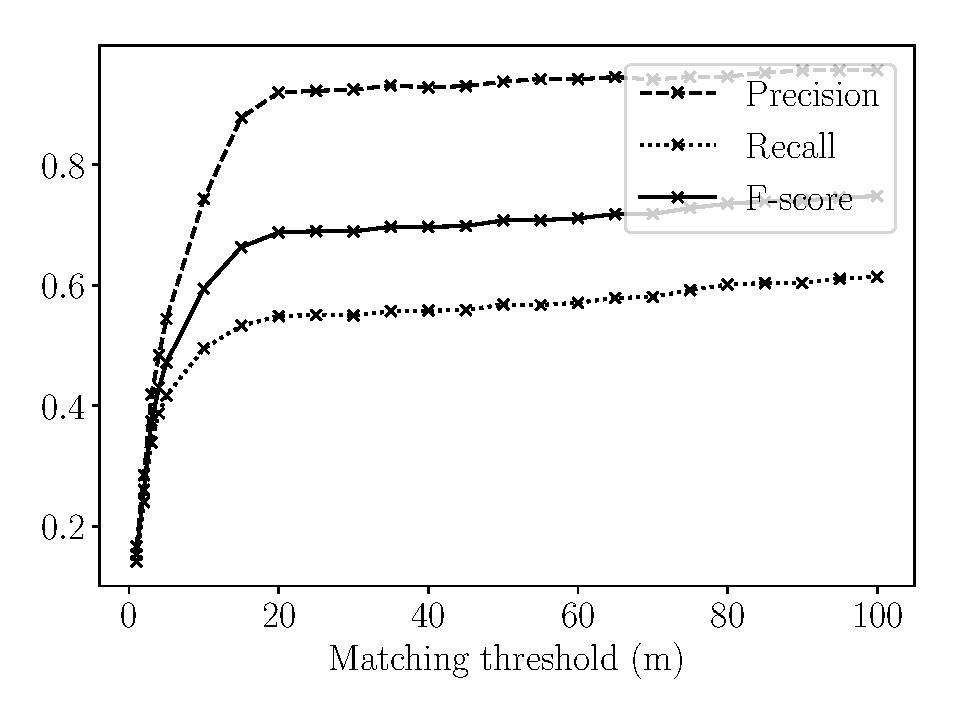
\includegraphics[width=0.6\linewidth]{Figures/Results/chicago/topo/match_dist_ch7ch1.pdf}\label{fig:results/topo_match_dist_ch7ch1} }%
  }
  \caption{GEO evaluation of the Chicago data sets using C7m and C1m as ground truth. The matching distance is varied from 1 to 100 meters and the sample spacing fixed to 5 m.}%
 \label{fig:results/topo_match_dist_chch}
\end{figure}

\begin{figure}[H]%

 \subfloat[\textit{\textit{C1m as base map.}}]{{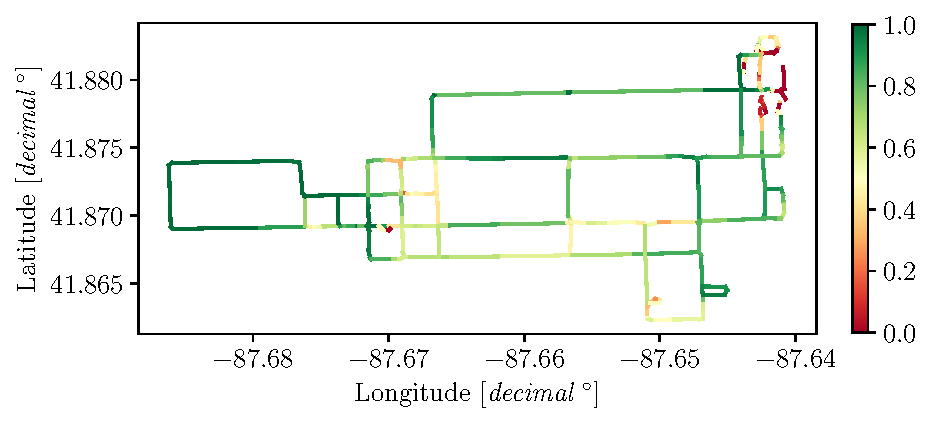
\includegraphics[width=0.8\linewidth]{Figures/Results/chicago/topo/signatures_ch1m7m.pdf} }}%
 
  \subfloat[\textit{C7m as base map.}]{{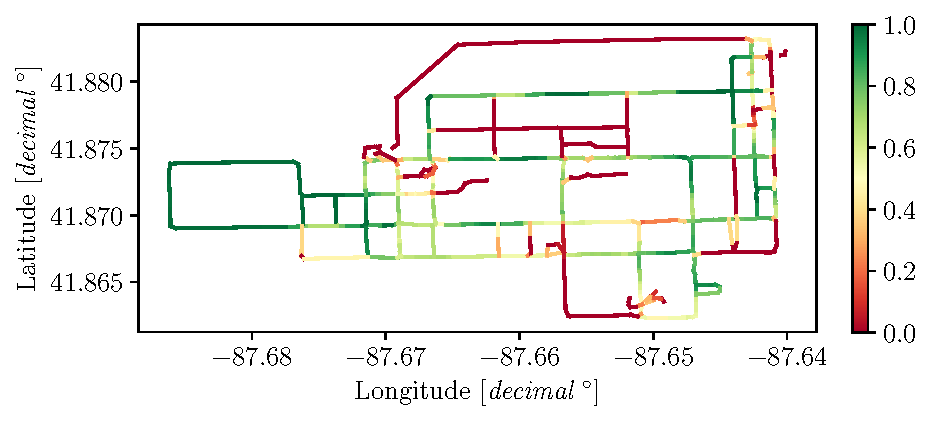
\includegraphics[width=0.8\linewidth]{Figures/Results/chicago/topo/signatures_ch7m1m.pdf} }}%
  
 \caption{Edge signatures for maps C1m and C7m calculated using TOPO.}%
 \label{fig:results/sig_topo_1m7m}
\end{figure}

\subsubsection{Path based}




%========================================================================%
\section{Map generation - Use less frequently sampled data}
%========================================================================%

In this section, only data from the Chicago data sets will be used, see section \ref{chp:data.sec:gpsdata.sec:chicago}. 

Discuss that we think 10 seconds is good enough.

%========================================================================%
\section{Scalability}
%========================================================================%

\begin{table}[H]
\centering
\caption{Execution times for the maps created with the Chicago 1 month and 7 month data set.}
\label{tab:results:exectimes_chicago}
\begin{tabular}{cc}
map name    & \begin{tabular}[c]{@{}c@{}}execution time\\ (hh:mm:ss)\end{tabular} \\ \hline
C1m         &                                                                     \\
C7m         &                                                                     \\
C1m$_{10}$  &                                                                     \\
C1m$_{20}$  &                                                                     \\
C1m$_{50}$  &                                                                     \\
C7m$_{0}$   &                                                                     \\
C7m$_{1}$   &                                                                     \\
C7m$_{2}$   &                                                                     \\ \hline
\end{tabular}
\end{table}


\% how long different steps in map generation takes

plot on 
 - time vs. \# gps points
 - time vs. km$^2$
 
%%%%%%%%%%%%%%%%%%%%%%%%
% less freq sampled data
%%%%%%%%%%%%%%%%%%%%%%%%

In table \ref{tab:exp_setup_102050_bbox} we can see that they cover more or less the same area. This is to be expected but also desired to confirm when starting to compare time scalability with respect to the amount data (number of samples), keeping the area of interest fixed. To get a better relative measure of the amount data we can compare the number of samples to the total road length. Let's denote the measure ``sample density''. \textbf{OBSOBS} 
% \ref{fig:results/c1m102050_time}
In figure \textbf{fig} we see the sample density plotted against execution time... 

\textbf{Since storing a lot of data requires a lot of storage, it is of great interest to understand how little data we can use to still get a map that represents the road network sufficiently accurately. REALLY GOOD QUESTION WHAT IS ACCURATELY ENOUGH. WE SAY, GIVEN OUR EVAL RESULTS THAT 10 s sampling.... }


%%%%%%%%%%%%%%%%%%%%%%%%
% three regions...
%%%%%%%%%%%%%%%%%%%%%%%%

%========================================================================%
\section{Map fuse}
%========================================================================%

In this section, only data from the Chicago data sets will be used, see section \ref{chp:data.sec:gpsdata.sec:chicago}. 

Short execution times, around 1 s.

% here we do fun stuffs (divide up 7m in 0, 1, 2)

%%%%%%%%%%%%%%%%%%%%%%%%
% OSM1m and OSM7m
%%%%%%%%%%%%%%%%%%%%%%%%
To test the performance of the method when using maps of higher quality and little noise we first attempt to fuse the two maps COSM12\_1m and COSM12\_7m. The result of using COSM12\_1m and COSM12\_7m respectively as base map is shown in figure \ref{fig:results/fusecosm1m7m}. The map fusion method performed well under these conditions and was less sensitive to parameter tuning.

\begin{figure}[H]%
 \centering
  \subfloat[\textit{\textit{COSM\_1M as base map.}}]{{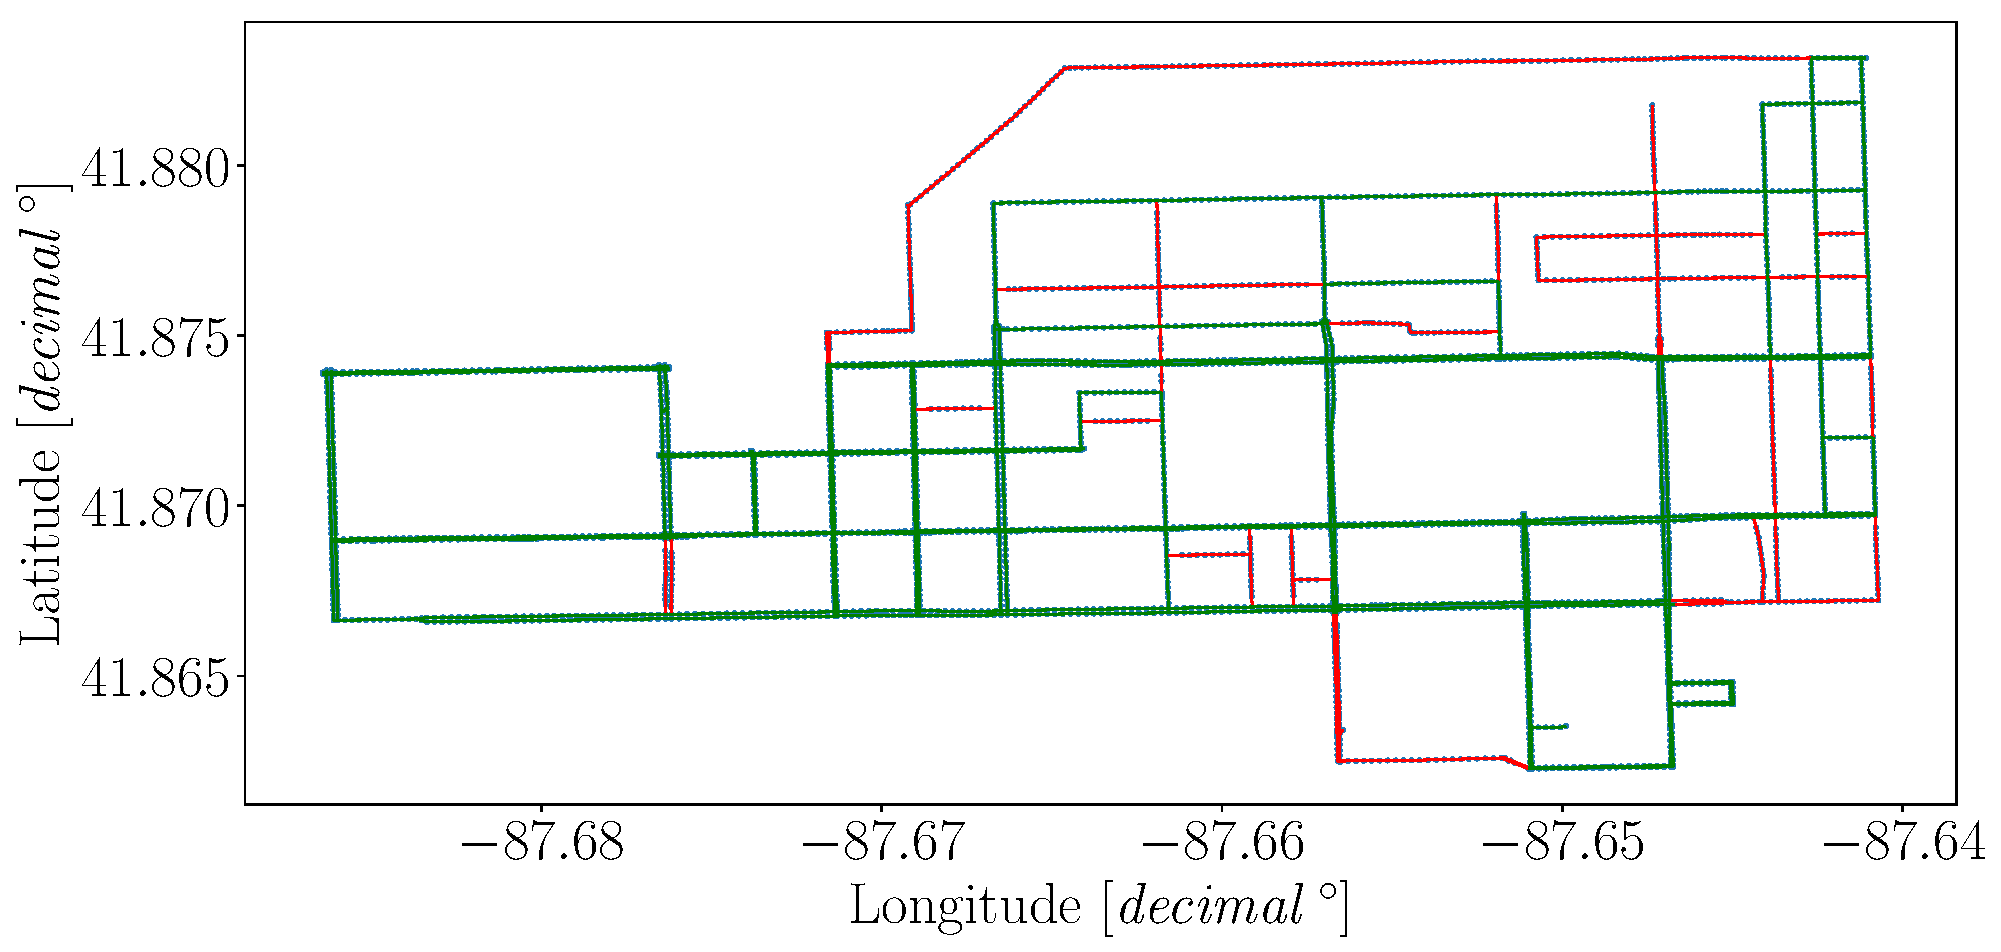
\includegraphics[width=0.8\linewidth]{Figures/Results/chicago/fuse/osm1osm7.pdf}\label{fig:results/fusecosm1m} }}% 

  \subfloat[\textit{COSM12$\_$7m as base map.}]{{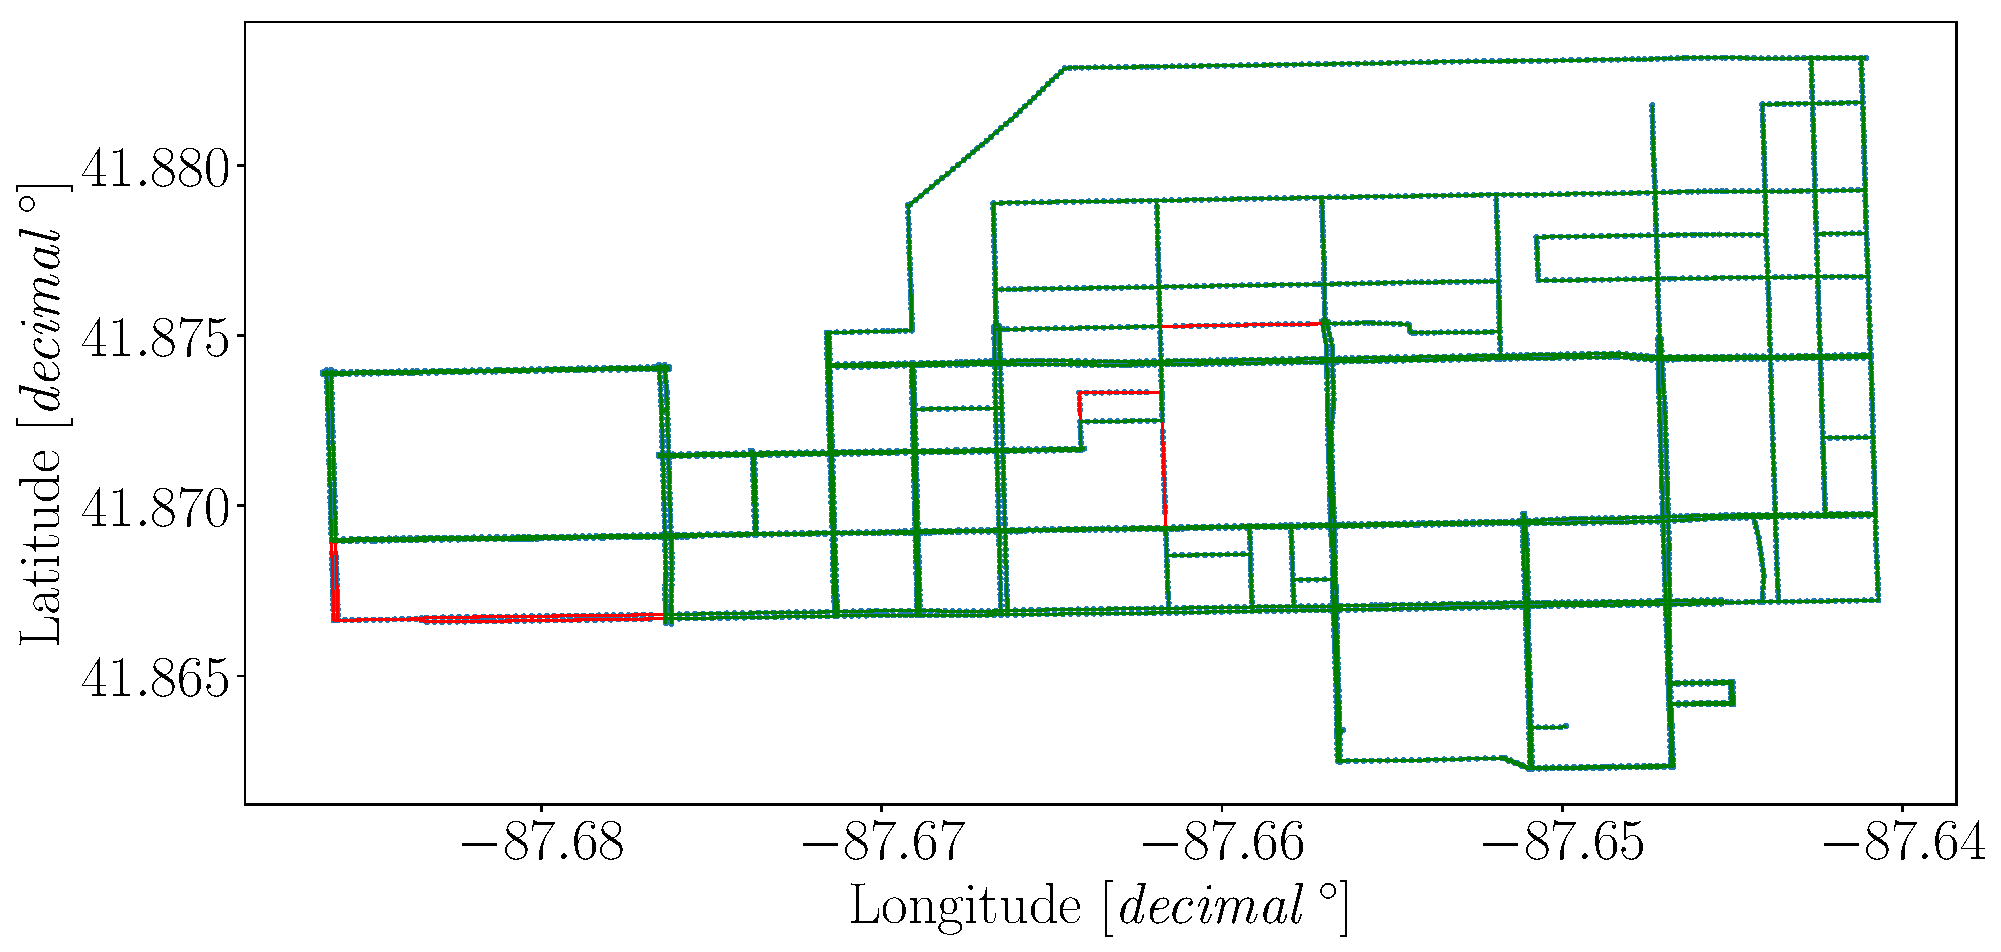
\includegraphics[width=0.8\linewidth]{Figures/Results/chicago/fuse/osm7osm1.pdf}\label{fig:results/fusecosm7m} }}%
  \caption{The result of fusing the two \ac{OSM} maps COSM12\_1m and COSM12\_7m.}%
 \label{fig:results/fusecosm1m7m}
\end{figure}



%%%%%%%%%%%%%%%%%%%%%%%%
% Ch1 and Ch7
%%%%%%%%%%%%%%%%%%%%%%%%
We next present the result of fusing the inferred maps C1m and C7m. In this case the result varied somewhat depending on the choice of parameter thresholds presented in section \ref{chp:experiments.sec:mapfuse.sub:dec.sub:add}.


%%%%%%%%%%%%%%%%%%%%%%%%
% three regions...
%%%%%%%%%%%%%%%%%%%%%%%%



%========================================================================%
\section{Lane level}
%========================================================================%

- BIld på färdig karta (använd final$\_$map.txt)
- Inzoomad bild (anders mailbild) -> problem på lanelevel
Det här är data som borde kunna ge oss lane level, tillräckligt hög precision på gps datan
Behövs tunas väldigt mycket. 
- visa bild på problem med cell size, behöver ha små boxar om vi ska kunna upplösa de olika lanesen. BLi boxarna för små för att få sammanhängande väg om för lite data + beräkningstungt